\subsection{Definir el archivo de rutas}
Definir el archivo de rutas de la aplicación sirve para saber qué direcciones y que comportamientos tendrá esta en su uso.
\\Las rutas de la aplicación son las indicadas en la figura \ref{rutas_aplicacion}.

\begin{figure}[ht]
    \centering
    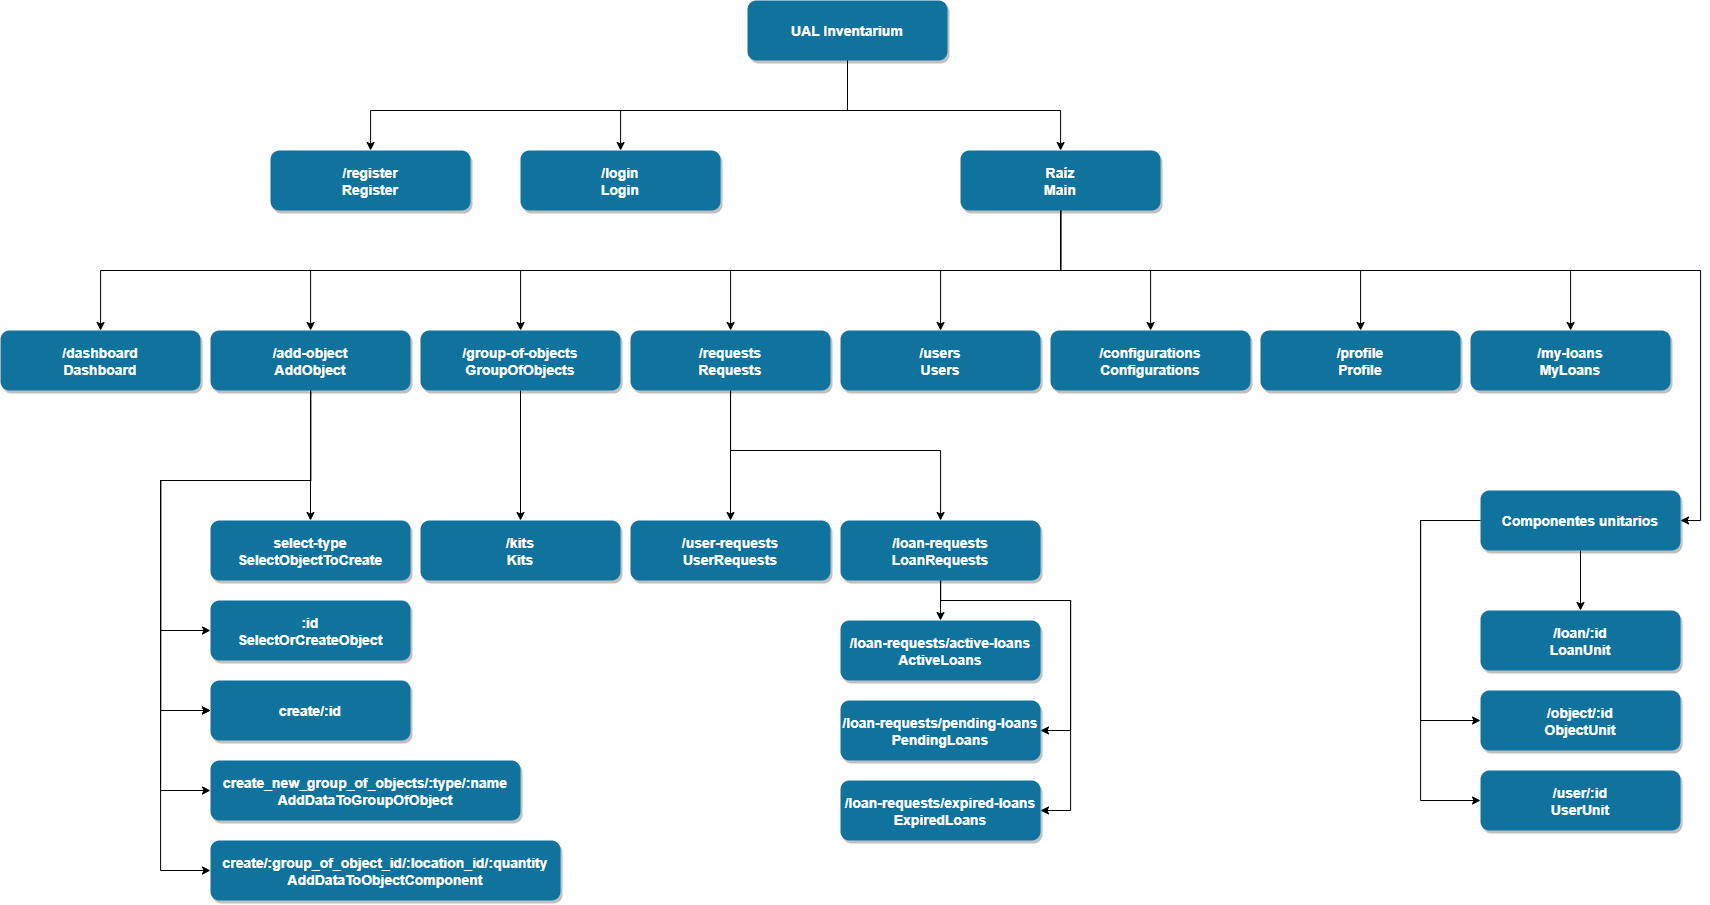
\includegraphics[width=\linewidth,keepaspectratio]{../contruccion_aplicacion/estructura_del_proyecto/app_routing.png}
    \caption{Rutas disponibles en la aplicación}\label{rutas_aplicacion}
\end{figure}

Las rutas de la aplicación tienen una correlación directa con el manejo de los componentes. Estas rutas se definen dentro del fichero \textit{app-routing.module.ts} que está dentro de \textit{app}.
\\Este archivo importa todos los componentes que vayan a utilizarse en las rutas. El comienzo del archivo consiste en definir una constante que se llamará routes y en la que irá toda la lógica de la aplicación:
\begin{verbatim}
    const routes: Routes = [
  {
    path: '', component: MainComponent,
    children: [
      { path: 'dashboard', component: DashboardComponent },
      {
        path: 'add-object', component: AddObjectComponent,
        children: [
          { path: 'select-type', component: SelectObjectToCreateComponent },
          .
          .
          .
\end{verbatim}
El archivo es bastante más extenso pero con este pequeño trozo pueden verse y explicarse los diferentes componentes que contiene.
\\Para definir una ruta de forma básica la estructura será la siguiente \textit{path: nombre\_de\_la\_ruta, component: nombre\_del\_componente} con esto al acceder a la ruta ya se mostraría dicho contenido.
\\Lo interesante que aporta Angular es la posibilidad de añadir hijos a estas rutas. Se hará llamando al atributo \textit{children: [array\_de\_rutas]}.
\\Esto es muy importante ya que el uso de hijos en las ruta hace que los componentes de rutas superiores no se descarguen. Se explicará mejor con el archivo \textit{MainComponent.html}:
\begin{verbatim}
<app-vertical-navbar></app-vertical-navbar>
<div class="page-content p-5" id="content">
    <!-- Toggle button -->
    <button id="sidebarCollapse" (click)="sidebarCollapse()" type="button"
    class="btn btn-light bg-white rounded-pill shadow-sm px-4 mb-4">
        <i class="fa fa-bars mr-2"></i>
        <small class="text-uppercase font-weight-bold">Toggle</small>
    </button>
    <router-outlet></router-outlet>
</div>
\end{verbatim}
Dentro del HTML se puede ver un componente llamativo: \textit{router-outlet}. Este está relacionado directamente con el routing que se tenga en la aplicación ya que es desde ahí donde se cargarán los hijos. La barra de navegación, por ejemplo, no desaparecería al acceder a \textit{/dashboard}.
\\Para realizar el importado de rutas dentro de Angular se llamará a \textit{\makeatletter@NgModule} al final del documento para que las exporte al componente principal.
\begin{verbatim}
    @NgModule({
        imports: [RouterModule.forRoot(routes)],
        exports: [RouterModule]
    })
\end{verbatim}